\chapter{Evaluation}
\label{ch:Evaluation}

\abstract{This chapter provides the analysis of the statistics gathered from the final implementations. As stated in the introduction the evaluation considers raw performance characteristics as well as developer productivity. Both areas are evaulated based on statistics from the previous chapter.
}

Preface: All data in this chapter was gathered from a high performance computer by courtesy of the research group \gls{wr}. The machine has access to four 12-core processors and 128 GB of memory. It is therefore ideal to compare shared memory performance on a large scale.

\section{Performance}
\label{sec:Evaluaton::Performance}

In \acrlong{hpc} the most important criteria when evaluating a language is performance. The important statistic that was tracked to compare performance is execution time. The benchmarks that were performed on the development laptop also roughly measured memory usage but that proved difficult to automate on the remote machine. It is therefore not directly included in this final evaluation. The first table shows the benchmark results in varying concurrency scenarios from singlethreaded execution up to 48 calculating in parallel.

\begin{table}[htb]
    \centering
    \begin{tabular}{rccc}
        \toprule
        % Header
            threads/goroutines
            & C
            & Go
            & Rust \\
        \midrule

            1
            & 21:51:18
            & 16:48:19
            & 14:15:06 \\

            2
            & 12:29:56
            & 10:21:36
            & 09:12:47 \\

            4
            & 07:16:34
            & 05:58:35
            & 05:09:56 \\

            8
            & 04:13:04
            & 03:01:54
            & 02:49:35 \\

            12
            & 03:17:28
            & 02:06:08
            & 01:55:33 \\

            24
            & 02:06:08
            & 01:13:47
            & 01:03:34 \\

            48
            & 01:21:58
            & 00:53:54
            & 00:44:54 \\

        \bottomrule
    \end{tabular}
    \caption{Execution time of the final applications (100.000 nodes)}
    \label{tb:final_execution_time}
\end{table}

These results already contain the first real surprise. C that was chosen as a comparitive baseline, since it is one of the two big programming languages in \gls{hpc}, is the slowest of the three compared languages in all configurations. In contrast the preliminary benchmarks on the development laptop showed C while not ahead at least on second place in the performance comparison. As briefly mentioned in the \hyperref[subsec:Implementation::ClusterPreparation::C]{previous chapter} this performance regression might have been caused by the two unoptimized libraries that were compiled on the development laptop and copied to the cluster. However this shows that C is still very much compiler and machine dependent.

In contrast the Go binary that was also compiled on the development laptop was executed without any changes on the target machine and shows great result even reaching similar performance to Rust in the high concurrency configurations. This shows that a garbage collected language is not immediately unsuitable for use in \gls{hpc}. Combined with the portability caused by full static linking Go might very well be suited for cluster computations on nodes with a minimum of system libraries installed.

Rust

Another important statistic to compare is the parallel speedup. A slow execution time alone does not mean a language is completely unfit for \gls{hpc} because the implementation might simply be flawed to begin with. If this is the case the application can still offer above average speedups making it viable for high concurrency scenarios. The following table highlights the achieved speedup for each language in the same configurations as above.

\begin{table}[htb]
    \centering
    \begin{tabular}{rccc}
        \toprule
        % Header
            threads/goroutines
            & C
            & Go
            & Rust \\
        \midrule

            1
            & \hspace{6pt}1.0000
            & \hspace{6pt}1.0000
            & \hspace{6pt}1.0000 \\

            2
            & \hspace{6pt}1.7486
            & \hspace{6pt}1.6221
            & \hspace{6pt}1.5469 \\

            4
            & \hspace{6pt}3.0037
            & \hspace{6pt}2.8119
            & \hspace{6pt}2.7590 \\

            8
            & \hspace{6pt}5.1816
            & \hspace{6pt}5.5432
            & \hspace{6pt}5.0424 \\

            12
            & \hspace{6pt}6.6406
            & \hspace{6pt}7.9941
            & \hspace{6pt}7.4003 \\

            24
            & 10.3961
            & 13.6659
            & 13.4520 \\

            48
            & 15.9980
            & 18.7072
            & 19.0445 \\

        \bottomrule
    \end{tabular}
    \caption{Parallel speedup of the final applications (100.000 nodes)}
    \label{tb:final_speedup}
\end{table}

\section{Additional metrics / productivity}
\label{sec:Evaluation::Metrics}

Next to performance the second main area evaluated in this thesis is developer productivity.

\begin{figure}
    \centering
    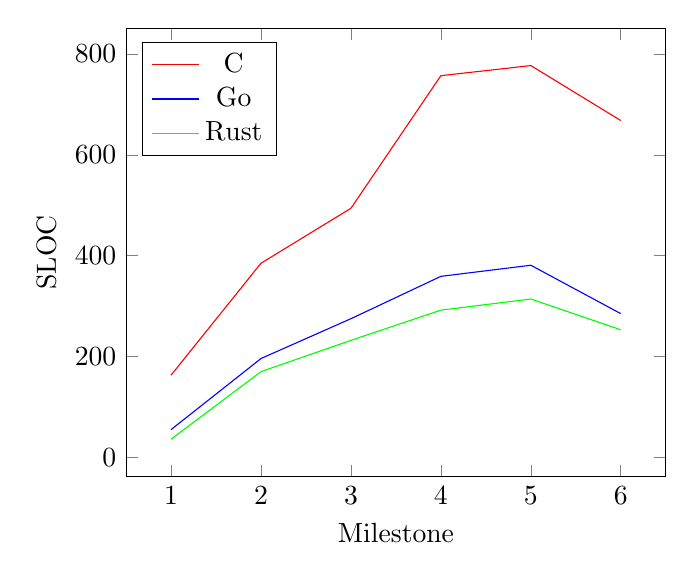
\begin{tikzpicture}
        \begin{axis}[
            xlabel={Milestone},
            ylabel={SLOC},
            xtick={1,2,3,4,5,6},
            legend pos=north west
        ]

        \addplot[red] plot coordinates {
            (1,163)
            (2,385)
            (3,494)
            (4,757)
            (5,777)
            (6,668)};
        \addlegendentry{C}

        \addplot[color=blue] plot coordinates {
            (1,55)
            (2,196)
            (3,275)
            (4,359)
            (5,381)
            (6,285)};
        \addlegendentry{Go}

        \addplot[color=green] plot coordinates {
            (1,36)
            (2,170)
            (3,232)
            (4,292)
            (5,314)
            (6,253)};
        \addlegendentry{Rust}
        \end{axis}
    \end{tikzpicture}
    \label{fig:sloc_graph}
    \caption{\gls{sloc} counts across the various milestones}
\end{figure}


\begin{figure}
    \centering
    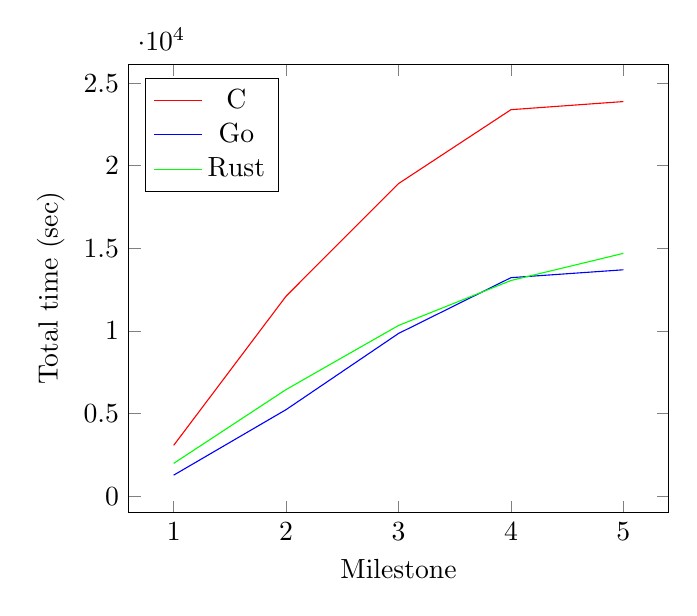
\begin{tikzpicture}
        \begin{axis}[
            xlabel={Milestone},
            ylabel={Total time (sec)},
            xtick={1,2,3,4,5,6},
            legend pos=north west
        ]

        \addplot[red] plot coordinates {
            (1,3078)
            (2,12110)
            (3,18920)
            (4,23392)
            (5,23883)};
        \addlegendentry{C}

        \addplot[color=blue] plot coordinates {
            (1,1276)
            (2,5242)
            (3,9851)
            (4,13227)
            (5,13703)};
        \addlegendentry{Go}

        \addplot[color=green] plot coordinates {
            (1,1989)
            (2,6457)
            (3,10335)
            (4,13055)
            (5,14698)};
        \addlegendentry{Rust}
        \end{axis}
    \end{tikzpicture}
    \label{fig:sloc_graph}
    \caption{Development time across the various milestones}
\end{figure}
